\section{问题四：垂荡与旋转阻尼联合优化}

\subsection{优化目标}

问题四沿用问题三的四自由度非线性几何耦合模型，将垂荡阻尼 $c_1$ 与旋转阻尼 $c_2$ 同时作为决策变量。瞬时输出功率定义为
\begin{equation}
  P(t)=c_1\dot z_z^2+c_2\dot\theta_z^2,
  \label{eq:p4_inst}
\end{equation}
其中 $\dot z_z$ 为振子沿中轴方向相对滑移速度，$\dot\theta_z$ 为振子相对浮子的纵摇角速度。优化目标为稳定周期区间内的平均总功率：
\begin{equation}
  \max_{0\le c_1,c_2\le 10^5}
  \bar P(c_1,c_2)=
  \frac{1}{T_2-T_1}\int_{T_1}^{T_2}
  \left(c_1\dot z_z^2+c_2\dot\theta_z^2\right)\,dt .
  \label{eq:p4_obj}
\end{equation}

\subsection{粗扫描与局部优化}

本文先在 $[0,10^5]\times[0,10^5]$ 上进行二维粗扫描，得到功率峰值的大致区域；再以粗扫描最优点为初值，采用 Powell 无导数方法局部精修。优化阶段使用较低精度的数值积分以提高效率，最终候选参数再用高精度长时间积分复算。功率统计时丢弃初始过渡过程，仅使用稳定区间计算平均值。

\begin{figure}[H]
  \centering
  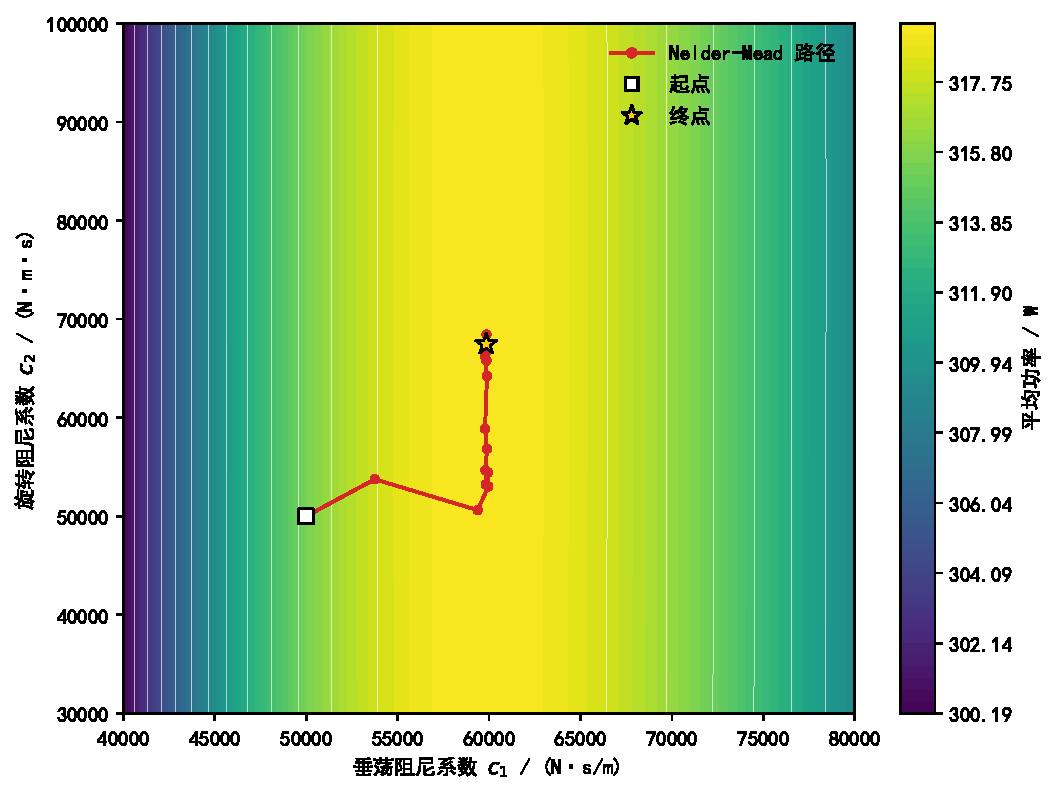
\includegraphics[width=0.78\textwidth]{fig_problem4_optimization_path_consistent.pdf}
  \caption{问题四垂荡阻尼与旋转阻尼的平均功率扫描结果}
  \label{fig:p4_surface}
\end{figure}

图~\ref{fig:p4_surface} 显示，功率对垂荡阻尼 $c_1$ 更敏感，而沿旋转阻尼 $c_2$ 方向变化较平缓。这与问题三中纵摇相对运动幅值较小的观察一致。

\subsection{最优结果与功率分解}

高精度复算得到
\begin{align*}
  c_1^\ast&=59846.67\,\mathrm{N\cdot s/m},\\
  c_2^\ast&=67472.34\,\mathrm{N\cdot m\cdot s},\\
  \bar P^\ast&=319.22345\,\mathrm{W}.
\end{align*}
其中垂荡平均功率为 $319.17646\,\mathrm{W}$，纵摇平均功率为 $0.04699\,\mathrm{W}$。因此本题参数下最优输出功率几乎全部由垂荡阻尼贡献。
\begin{figure}[H]
  \centering
  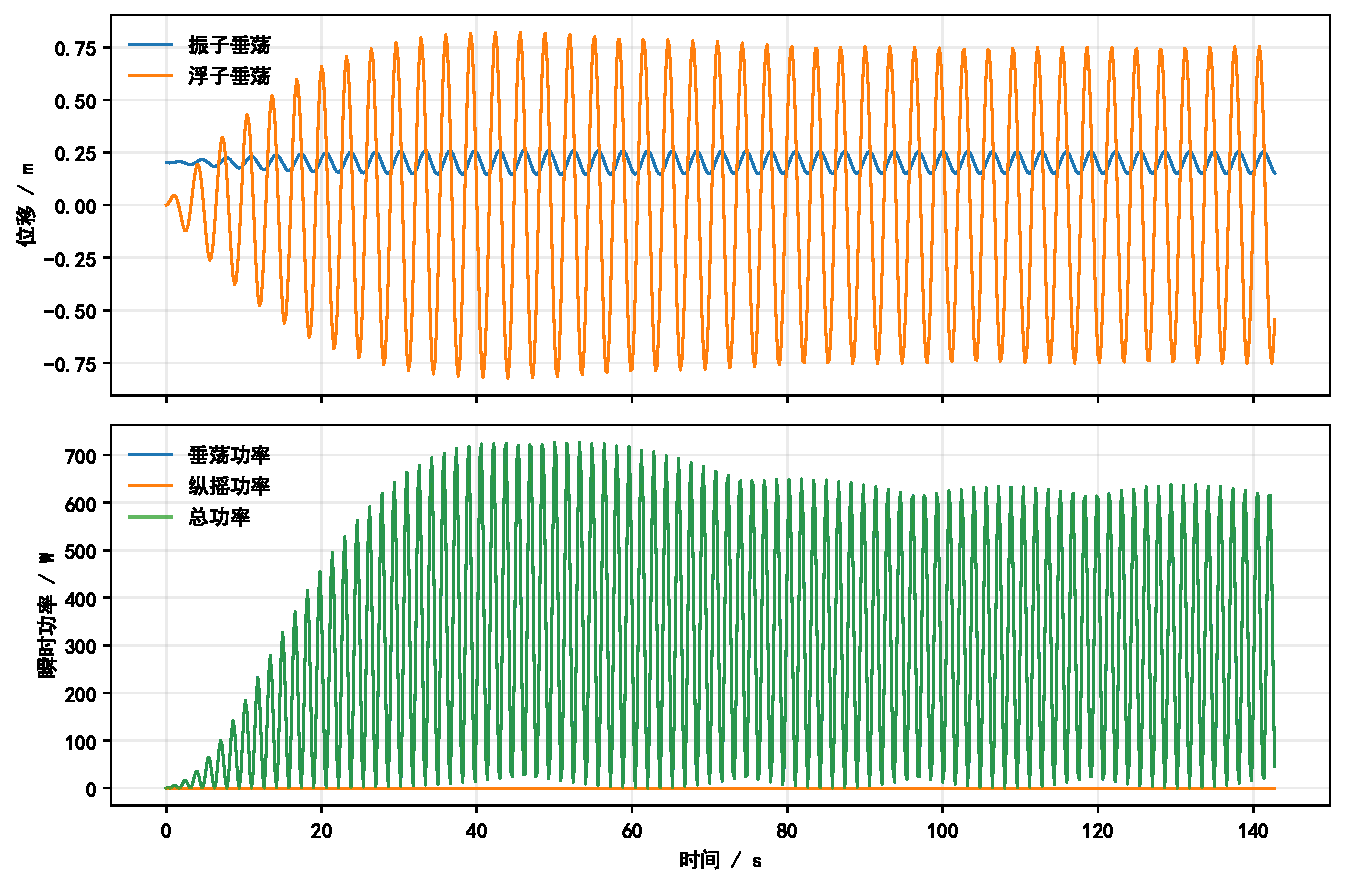
\includegraphics[width=0.90\textwidth]{fig_problem4_response_power.pdf}
  \caption{问题四最优阻尼参数下的响应与功率分解}
  \label{fig:p4_response}
\end{figure}
